% !TeX encoding = UTF-8
% !TeX program = xelatex
% !TeX spellcheck = en_US

\documentclass{cjc}

\usepackage{booktabs}
\usepackage{algorithm}
\usepackage{algorithmic}
\usepackage{siunitx}

\classsetup{
  % 配置里面不要出现空行
  title        = {题目},
  title*       = {Title},
  authors      = {
    author1 = {
      name         = {作者名},
      name*        = {name},
      affiliations = {aff1},
      biography    = {},
      biography*   = {},
      email        = {**************},
      classname    = {自动化XX班},
      student-id = {UXXXXXXX},  % 学号
    }
  },
  affiliations = {
    aff1 = {
      name  = {华中科技大学,人工智能与自动化学院},
      name* = {School of Articial Intelligence and Automation, Huazhong University of Science and Technology},
    },
  },
  abstract     = {
    中文摘要内容置于此处(英文摘要中要有这些内容)
  },
  abstract*    = {Abstract (英文摘要,内容包含中文摘要的内容). },
  keywords     = {关键词, 关键词, 关键词, 关键词},
  keywords*    = {key word, key word, key word, key word},
}

\newcommand\dif{\mathop{}\!\mathrm{d}}

% hyperref 总是在导言区的最后加载
\usepackage{hyperref}


\begin{document}

\maketitle


\section{介绍}

介绍\cite{article_example}


\section{方法}

\subsection{二级标题}

\subsubsection{三级标题}

正文部分

文件排版采用 TeX Live。

正文文字要求语句通顺,无语法错误,结构合理,条理清楚,不影响审稿人、读者阅读理解全文内容。以下几类问题请作者们特别注意:

1)文章题目应明确反映文章的思想和方法;文字流畅,表述清楚;

2)中文文字、英文表达无语法错误;

3)公式中无符号、表达式的疏漏,没有同一个符号表示两种意思的情况;

4)数学中使用的符号、函数名用斜体;

5)使用的量符合法定计量单位标准;

6)矢量为黑体,标量为白体;

7)变量或表示变化的量用斜体;

8)图表规范,量、线、序无误,位置正确(图表必须在正文中有所表述后出现,即…如图1所示)(注意纵、横坐标应有坐标名称和刻度值)。

9)列出的参考文献必须在文中按顺序引用,即参考文献顺序与引用顺序一致,各项信息齐全(格式见参考文献部分);

10)首次出现的缩写需写明全称,首次出现的符号需作出解释。

11)图的图例说明、坐标说明全部用中文或量符号。

12)图应为矢量图。

13)表中表头文字采用中文。

14)公式尺寸:

标准:10.5磅

下标/上标:5.8磅

次下标/上标:4.5磅

符号:16磅

次符号:10.5磅

15)组合单位采用标准格式,如:“pJ/bit/m4”应为“\si{pJ/(bit.m^4)}”


\begin{theorem}
  定理内容。
  “定义”、“假设”、“公理”、“引理”等的排版格式与此相同,详细定理证明、公式可放在附录中。
\end{theorem}

\begin{proof}
  证明过程.
\end{proof}

\begin{figure}[htb]
  \centering
  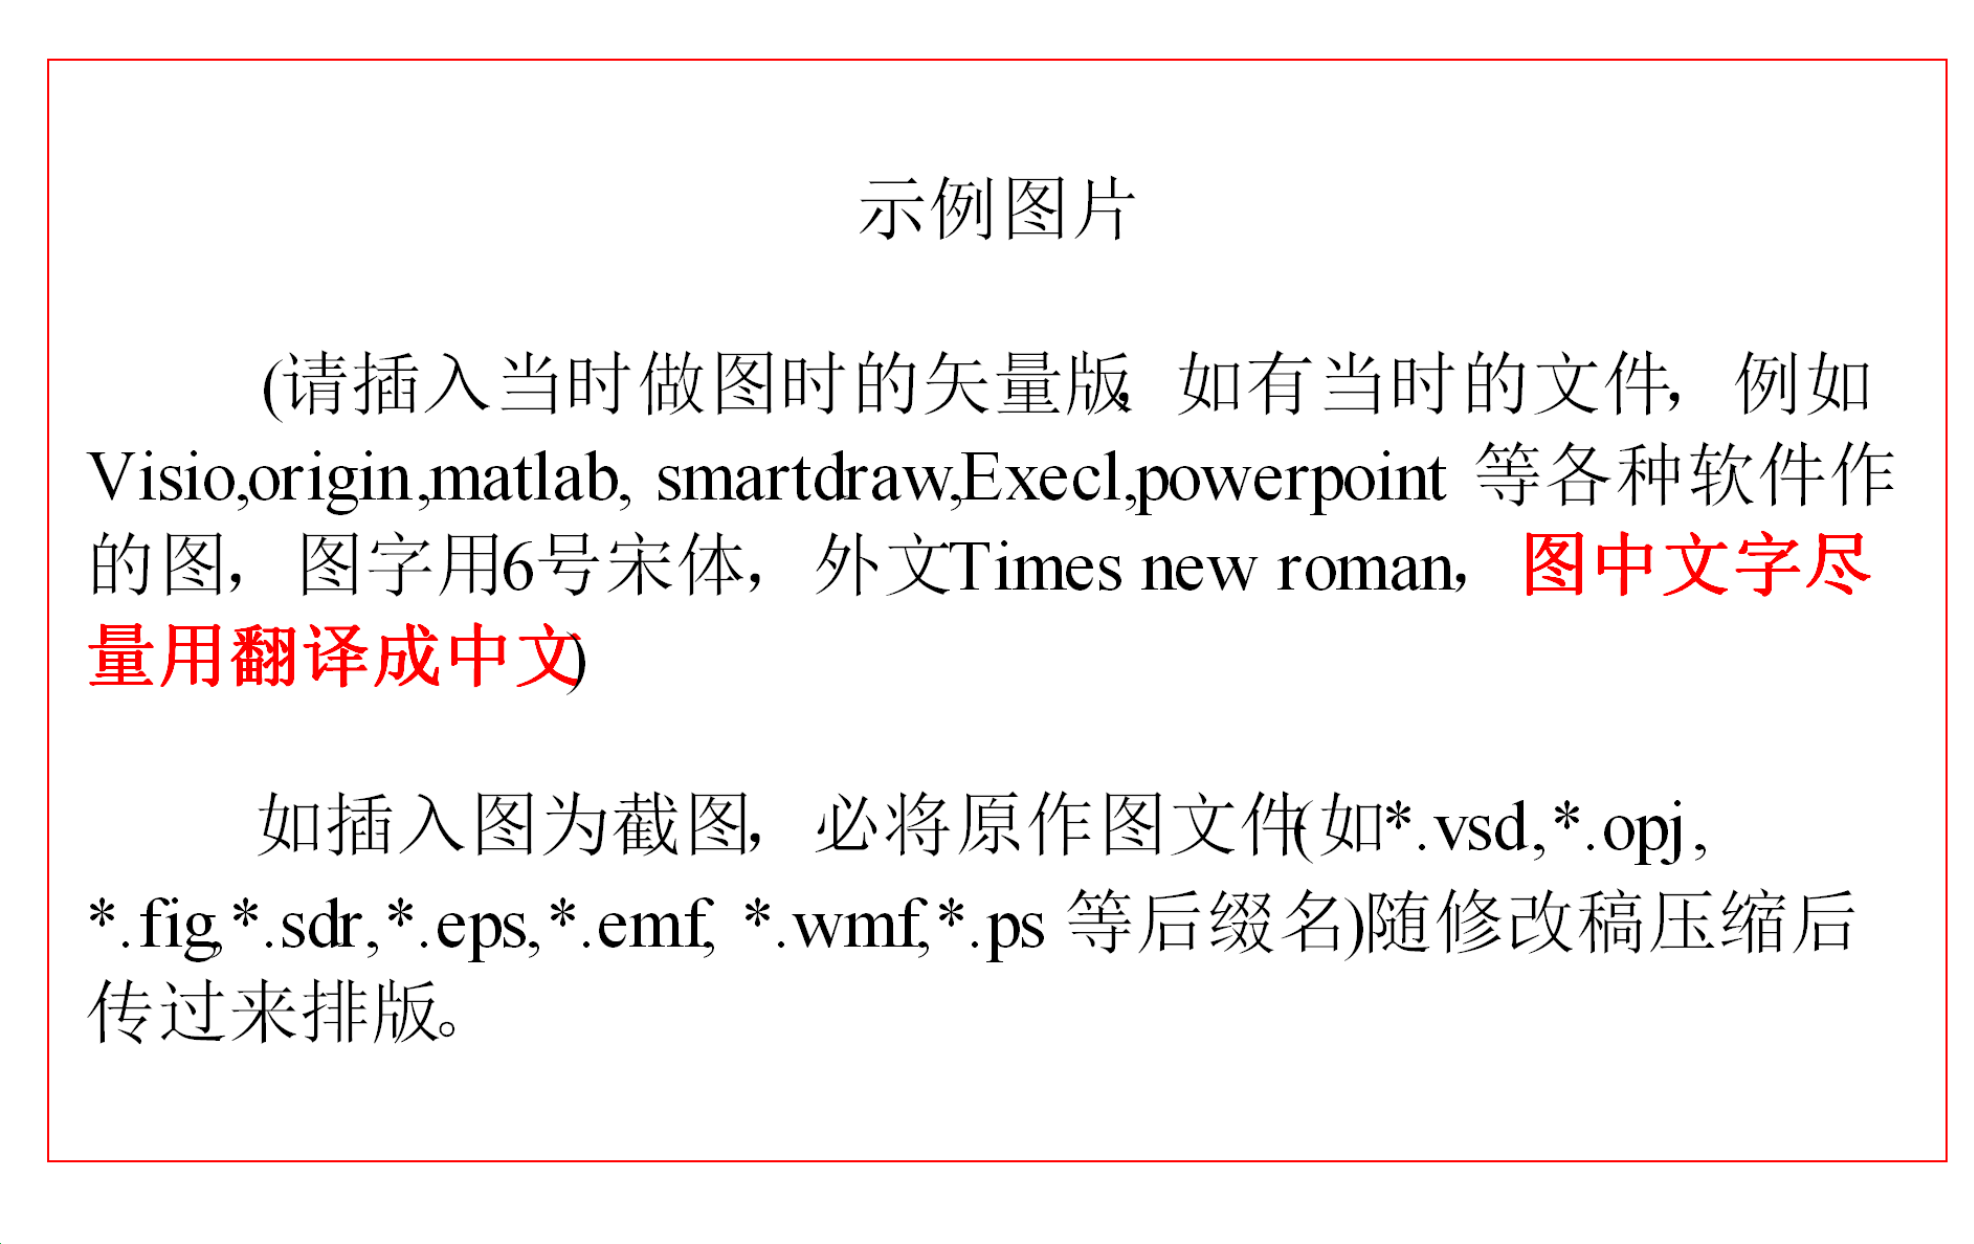
\includegraphics[width=\linewidth]{figures/fig1.png}
  \caption{图片说明 图中的子图要有子图说明}
\end{figure}

\begin{table}[htb]
  \centering
  \caption{表说明}
  \small
  \begin{tabular}{cc}
    \toprule
    示例表格 & 第一行为表头,表头要有内容 \\
    \midrule
    & \\
    \midrule
    & \\
    \bottomrule
  \end{tabular}
\end{table}


\begin{algorithm}
  \caption{算法名称}
  \small
  \begin{algorithmic}
    \REQUIRE $n \geq 0 \vee x \neq 0$
    \ENSURE $y = x^n$
    \STATE $y \leftarrow 1$
    \IF{$n < 0$}
      \STATE $X \leftarrow 1 / x$
      \STATE $N \leftarrow -n$
    \ELSE
      \STATE $X \leftarrow x$
      \STATE $N \leftarrow n$
    \ENDIF
    \WHILE{$N \neq 0$}
      \IF{$N$ is even}
        \STATE $X \leftarrow X \times X$
        \STATE $N \leftarrow N / 2$
      \ELSE[$N$ is odd]
        \STATE $y \leftarrow y \times X$
        \STATE $N \leftarrow N - 1$
      \ENDIF
    \ENDWHILE
  \end{algorithmic}
\end{algorithm}

\begin{procedure}
  \caption{过程名称}
  \small
  \begin{algorithmic}
    \REQUIRE
    \ENSURE
    \STATE \COMMENT{方法过程描述字体为小5号宋体,IF 、THEN等伪代码关键词全部用大写字母,变量和函数名称用斜体}
  \end{algorithmic}
\end{procedure}

\section{结论}

\section{总结}


\nocite{*}
\bibliographystyle{cjc}
\bibliography{example}

\end{document}
